\documentclass[a4paper,openright, 10pt]{article}
\usepackage[utf8]{inputenc}
\usepackage{graphicx}
\usepackage{tikz}
\usetikzlibrary{datavisualization}
\usetikzlibrary{datavisualization.formats.functions}

\graphicspath{ {./Images/} }

\usepackage{fullpage}
\newcommand{\ssection}[1]{%
\section[#1]{\centering\normalfont\scshape #1}}
\newcommand{\ssubsection}[1]{%
\subsection[#1]{\bfseries\normalfont\scshape #1}}
\newcommand{\ssubsubsection}[1]{%
\ssubsubsection[#1]{\bfseries\normalfont\scshape #1}}

\title{Folium of Descartes}
\author{Lauren Bourque }
\date{December 2018}

\begin{document}

\maketitle

\ssection{Introduction}
\section*{The Problem}
$$x^3+y^3=3xy$$ 
\section*{A Brief Backstory}
The problem first came about in the 1600's when Descartes challenged fellow mathematician, Pierre de Fermat, to  find the slope of the tangent line for any point over the curve. This is how the folium earned its name. A folium is a cubic curve with a single loop, one node (point where it crosses itself), and a slant asymptote. Using this information, let's explore the depth of what this information means about the curve as a whole.
\ssection{Solving the Problem}
\section*{Converting to Parametric Form}
We're given the problem in rectangular form, or solely in terms of $x$ and $y$. To understand how the graph moves over time, $t$, we must convert it to parametric form.
$$x^3+y^3=3xy$$
Let's use $y=tx$ to convert the equation to parametric form.
$$x^3+(tx)^3=3x\cdot tx$$
$$x^3+t^3x^3=3tx^2$$
Factor out $t^3$ from the left side.
$$x^3(1+t^3)=3tx^2$$
Divide both sides by $x^2$
$$\frac{x^3(1+t^3)}{x^2}=\frac{3tx^2}{x^2}$$
$$x(1+t^3)=3t$$
Divide by $(1+t^3)$ to isolate x.
$$x=\frac{3t}{t^3+1}$$
Now, we can use our prior knowledge of $y=tx$ to substitute$\frac{y}{t}$ in for x.
$$\frac{y}{t}=\frac{3t}{t^3+1}$$
Multiply both sides by $t$ to isolate y.
$$y=\frac{3t^2}{t^3+1}$$
\ssection{Exploring Deeper}
\section*{Graphing}
Now that we have the problem in parametric form, we can graph it and see how it changes over time.
\begin{center}
    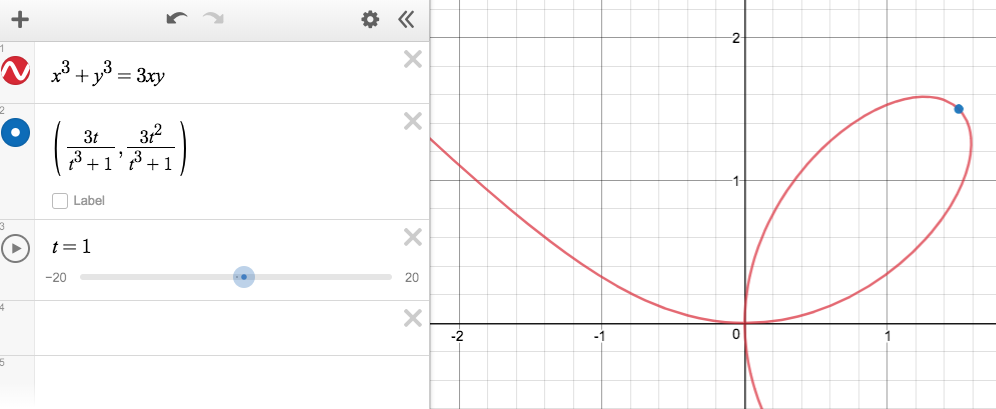
\includegraphics[scale=0.5]{graph}
\end{center}
This is what the folium looks like as graphed. As we can see, it appears to be a symmetrical loop. 
\begin{center}
    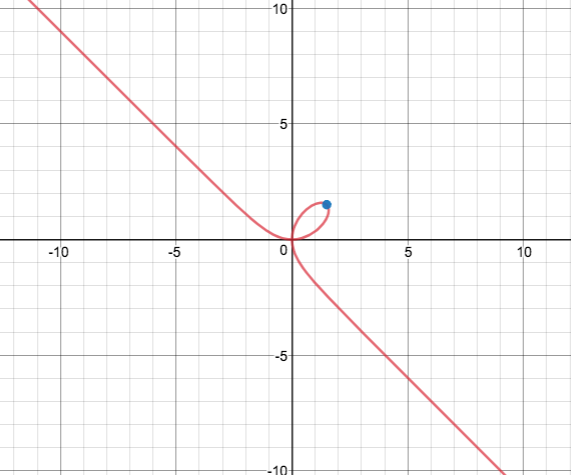
\includegraphics[scale=0.5]{graph1}
\end{center}
If we take a closer look at the graph, we can see that the graph appears to approach an asymptote over time. From this, we could easily assume that over time, a point would travel perfectly along this line with no interruptions and continue around the loop with its x values constantly approaching infinity or negative infinity. However, this is not the case.
\section*{The Beginning of the Graph}
To better understand this graph, let's look at where it starts and ends. Let's try substituting 0 in for t.
$$x(0)=\frac{3(0)}{0^3+1}$$
$$x(0)=0$$
$$y(0)=\frac{3(0)^2}{0^3+1}$$
$$y(0)=0$$
So, we can see that at the beginning of the graph, or $t=0$, the graph begins at the origin. Let's examine this point on the graph.
\begin{center}
    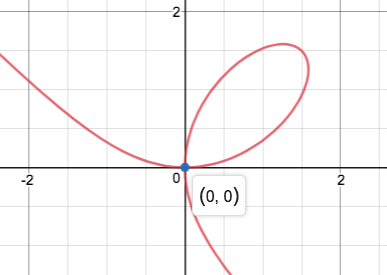
\includegraphics[scale=0.5]{graph2}
\end{center}
Sure enough, the graph confirms this. So, the better question is: where does the graph end?
\section*{End Behavior and Limits}
The end behavior of the graph is more difficult to understand because it's different as t approaches a positive or negative value. To see how the graph changes as t approaches positive infinity, let's choose a very high number and substitute it in our parametric equation. This will produce a point that we can graph and be able to see how the graph acts.
$$x(10,000)=\frac{30,000}{10,000^3+1}$$
$$x(10,000)=0.00000003$$
$$y(10,000)=\frac{3\cdot 10,000^2}{10,000^3+1}$$
$$y(10,000)=0.0003$$
These numbers are very small. From this, we can conclude that they'll continue to grow smaller, continuously approaching zero. Let's graph the point and see how the graph behaves.
\begin{center}
    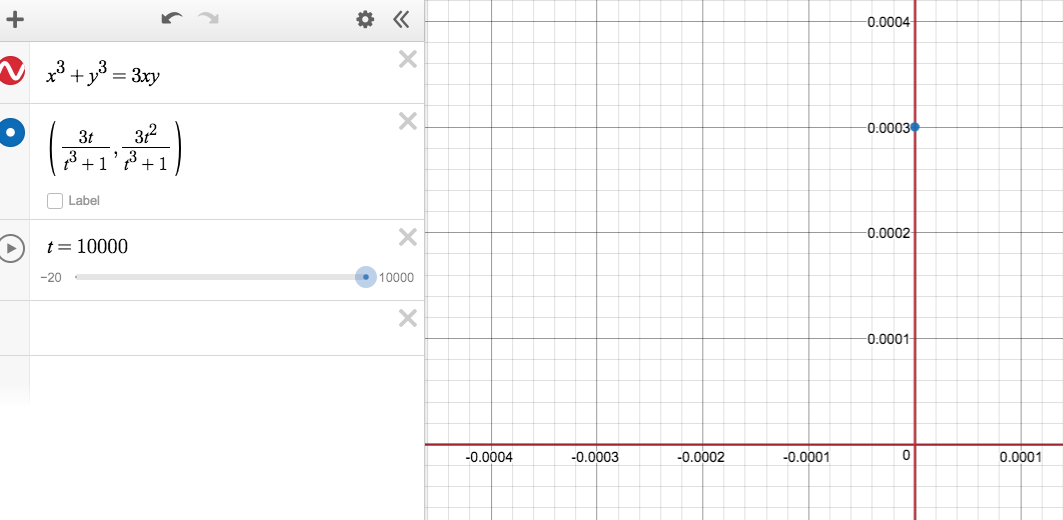
\includegraphics[scale=0.5]{graph3}
\end{center}
We can see that the graph is at this point and still hasn't reached zero, even though the t value is quite high. Let's try the same thing, but for a very low negative number.
$$x(-10,000)=\frac{-30,000}{-10,000^3+1}$$
$$x(-10,000)=0.00000003$$
$$y(-10,000)=\frac{3\cdot -10,000^2}{-10,000^3+1}$$
$$y(-10,000)=-0.0003$$
These numbers are very small. They're the same numbers that we got when we substituted positive 10,000 into the parametric equations, except the y value is negative this time. This gives an indication that the graph may be symmetrical in many ways.
\begin{center}
    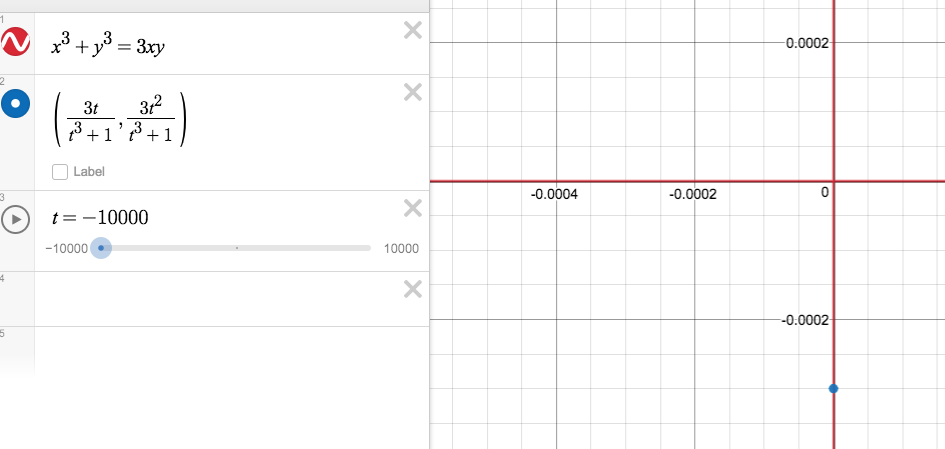
\includegraphics[scale=0.5]{graph4}
\end{center}
As we can see, the graph has the same behavior as the image above, except that it approaches zero from the negatives instead of the positives. So, from here, we can conclude:
$$\lim_{t\to\infty} x^3+y^3=3xy$$
Equals $0^+$.
$$\lim_{t\to-\infty} x^3+y^3=3xy$$
Equals $0^-$\\
\section*{Discontinuities}
When we look at the parametric equations $x=\frac{3t}{t^3+1}$ and $y=\frac{3t^2}{t^3+1}$, we can see that if we set the denominator of each fraction equal to zero, we would get a value of -1 for t. Using our prior mathematical knowledge, from this we should be able to conclude that there can never be values of x and y exactly at t=-1 because if t=-1, the denominator would equal zero. This would mean that t=-1 must be an asymptote that a point on the graph never touches.
\begin{center}
    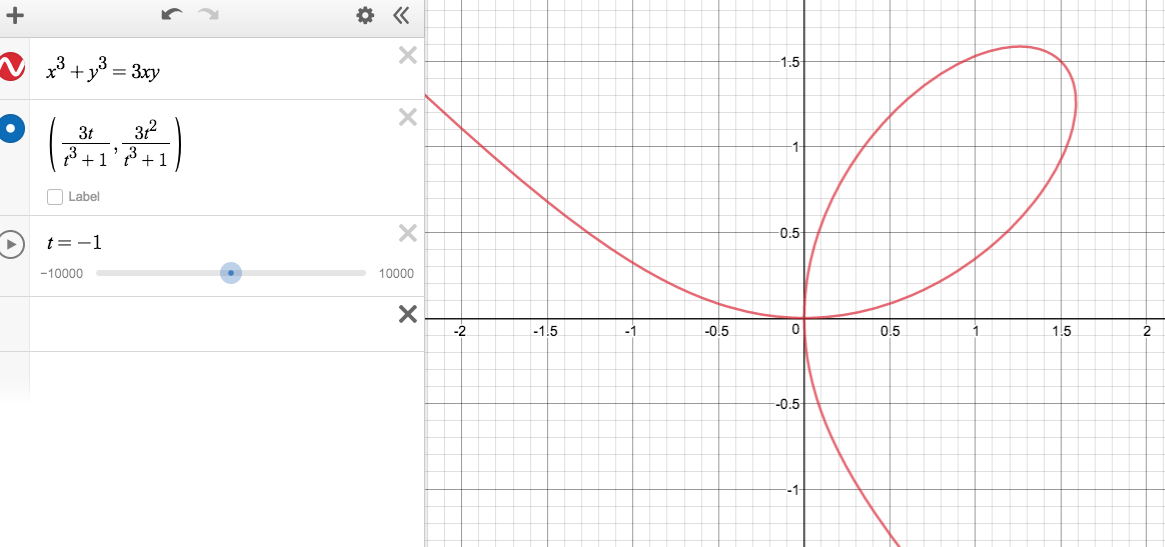
\includegraphics[scale=0.45]{graph5}
\end{center}
Since there appears to be no point on the graph exactly at t=-1, let's look at what happens to the graph as t approaches negative one from the right and the left. 
$$x=\frac{3t}{t^3+1}$$
$$\lim_{t\to-1^+} \frac{3t}{t^3+1}$$
To evaluate this limit, we have to imagine what would happen if we substituted a number slightly larger than -1 in for t. Let's try substituting in -0.99 and -0.999 to see what happens to the value of x as we get closer to -1 from the right. 
$$\frac{3(-0.99)}{(-0.99)^3+1}=-99.997$$
We see that this is a very negative number. Let's see what happens when we get slightly closer to -1 from the right.
$$\frac{3(-0.999)}{(-0.999)^3+1}=-999.9997$$
This number is even closer to negative infinity than the last. Based on this, we can conclude that as t approaches -1 from the right, x approaches negative infinity. Therefore:
$$\lim_{t\to-1^+} x=-\infty$$
Now let's see how y behaves.
$$y=\frac{3t^2}{t^3+1}$$
$$\lim_{t\to-1^+} \frac{3t^2}{t^3+1}$$
Let's substitute in the same two t values that we used before.
$$\frac{3(-0.99)^2}{-0.99^3+1}=98.997$$
We can see that this is a large positive number. Let's see what happens as we get closer to t=-1.
$$\frac{3(-0.999)^2}{-0.999^3+1}=998.9997$$
This number is even closer to infinity, so we can conclude that as t approaches negative one from the right, y approaches positive infinity. Therefore:
$$\lim_{t\to-1^+} y=\infty$$
Now let's see what happens as we approach t=-1 from the left.
$$x=\frac{3t}{t^3+1}$$
$$\lim_{t\to-1^-} \frac{3t}{t^3+1}$$
Let's try substituting in -1.01 and -1.001 to see what happens as we get slightly closer to t=-1 from the left.
$$\frac{3(-1.01)}{-1.01^3+1}=99.997$$
This is a large positive number. Let's try -1.001 now.
$$\frac{3(-1.001)}{-1.001^3+1}=999.9997$$
This number is even larger, so we can conclude that as t approaches -1 from the left, x approaches infinity. Therefore:
$$\lim_{t\to-1^-} x=\infty$$
Now, let's see how y changes.
$$y=\frac{3t^2}{t^3+1}$$
$$\lim_{t\to-1^-} \frac{3t^2}{t^3+1}$$
Let's substitute in -1.01.
$$\frac{3(-1.01)^2}{-1.01^3+1}=-100.997$$
This is a very negative number. Let's try -1.001.
$$\frac{3(-1.001)^2}{-1.001^3+1}=-1000.9997$$
This number is even closer to negative infinity, so we can conclude that as t approaches -1 from the left, y approaches negative infinity. Therefore:
$$\lim_{t\to-1^-} y=-\infty$$
Let's try looking at the graph to be able to see how this change happens over time. 
\begin{center}
    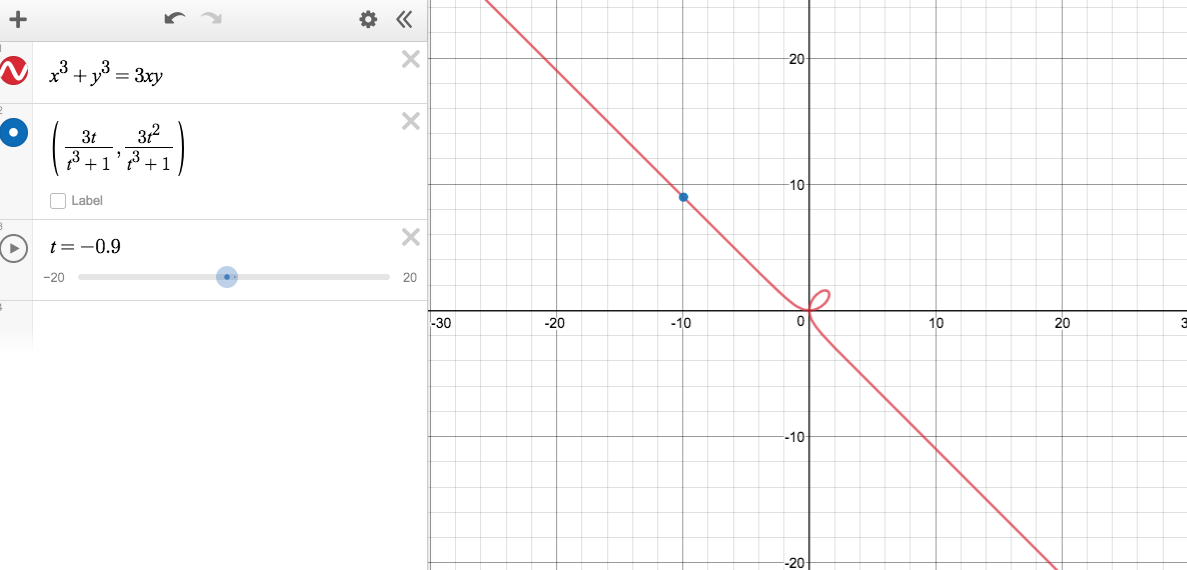
\includegraphics[scale=0.45]{graph10}
\end{center}
The point on the graph at the moment is -0.9; a point that approaches negative one from the right. We can see that it's in the second quadrant. As t gets closer to -1, that point moves left on the graph, extending to negative infinity for x and positive infinity for y, proving that our conclusions were correct. Let's try looking at a point on the graph that approaches -1 from the left.
\begin{center}
    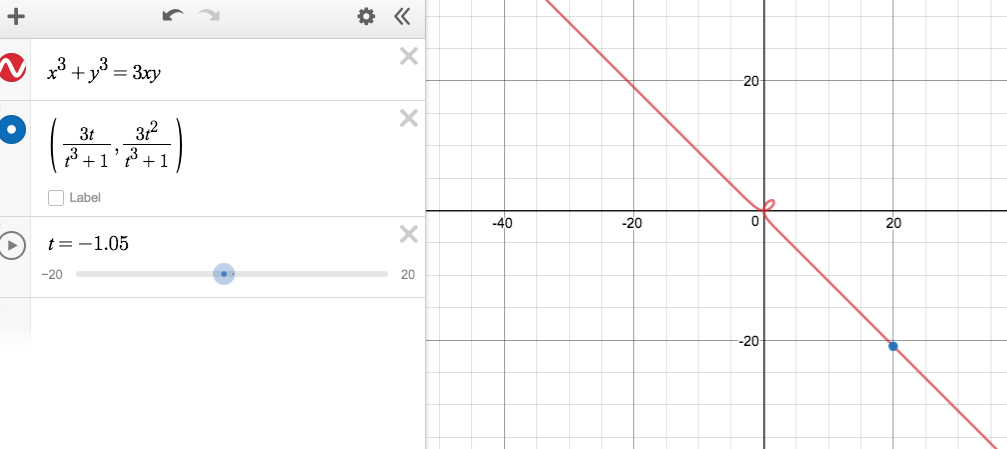
\includegraphics[scale=0.45]{graph11}
\end{center}
The point on the graph at this moment is -1.05; a point that approaches negative one from the left. It's in the fourth quadrant. As t gets closer to -1, that point moves right on the graph, extending to positive infinity for x and negative infinity for y, proving that our conclusions were correct. Since we now understand the behavior of the graph t approaches negative one from the left and right, we can only assume that at t=-1, the ends of the graph that stretch out end up connecting, or at least attempting to connect. 
\section*{The Coordinate of the Loop}
In order to understand this equation even better, we should explore what the coordinate of the loop is and see if it continues to reflect the symmetry that we're seeing in the graph. If the graph continues to be symmetrical along the $y=x$ line, we can use this knowledge to find the tip of the loop because the tip of the loop would be a point on this line. Let's use this knowledge of $y=x$ and set the x and y parametric equations equal to each other.
$$\frac{3t}{t^3+1}=\frac{3t^2}{t^3+1}$$
Multiply both sides by $t^3+1$
$$3t=3t^2$$
Divide both sides by $3t$
$$1=t$$
Now, let's take the t value that we found and substitute it into the x and y parametric equations.
$$x(1)=\frac{3(1)}{1^3+1}$$
$$x(1)=1.5$$
$$y(1)=\frac{3(1)^2}{1^3+1}$$
$$y(1)=1.5$$
Therefore, the tip of the loop appears to be at the point (1.5,1.5). Let's check the graph to make sure this is correct.
\begin{center}
    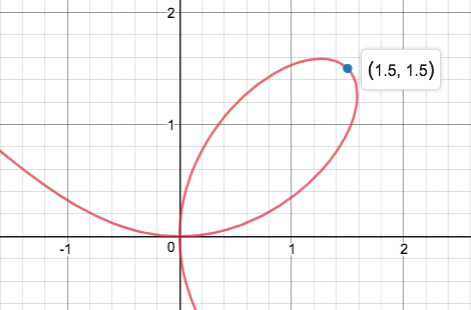
\includegraphics[scale=0.5]{graph6}
\end{center}
Eureka!
\ssection{Derivatives}
\section*{Finding Derivatives}
To be able to explore tangent lines of the graph, we should find $\frac{dy}{dt}$,$\frac{dx}{dt}$, and $\frac{dy}{dx}$.\\
To find $\frac{dy}{dx}$, we'll have to use implicit differentiation on the original equation.
$$x^3+y^3=3xy$$
$$3x^2+3y^2\frac{dy}{dx}=y\cdot3 +3x\frac{dy}{dx}$$
Divide by 3.
$$x^2+y^2\frac{dy}{dx}=y+x\frac{dy}{dx}$$
Work to get everything being multiplied by $\frac{dy}{dx}$ to one side of the equation and factor out $\frac{dy}{dx}$.
$$x^2-y=\frac{dy}{dx}(x-y^2)$$
Isolate $\frac{dy}{dx}$
$$\frac{x^2-y}{x-y^2}=\frac{dy}{dx}$$
Now, let's find $\frac{dy}{dt}$, using the parametric equation for y.
$$\frac{t^3+1(6t)-3t^2(3t^2)}{(t^3+1)^2}$$
$$\frac{6t-3t^4}{(t^3+1)^2}$$
Now, let's find $\frac{dx}{dt}$, using the parametric equation for x.
$$\frac{t^3+1(3)-3t(3t^2)}{(t^3+1)^2}$$
$$\frac{3-6t^3}{(t^3+1)^2}$$
Let's use these two derivatives to find y' in terms of t.
$$\frac{dy}{dx}=\frac{\frac{6t-3t^4}{(t^3+1)^2}}{\frac{3-6t^3}{(t^3+1)^2}}$$
We can cancel out the $(t^3+1)^2$ and we're left with
$$y'=\frac{6t-3t^4}{3-6t^3}$$
Simplify
$$y'=\frac{t(2-t^3)}{1-2t^3}$$
\section*{Using Derivatives to Find Tangent Lines}
Let's use the derivatives to find horizontal and vertical tangent lines and the tangent line at the tip of the loop.\\
First, to find the horizontal tangent line, we'll have to find when $\frac{dy}{dt}$ is 0.
$$\frac{dy}{dt}=0$$
$$0=\frac{6t-3t^4}{(t^3+1)^2}$$
Multiply both sides by the denominator.
$$0=6t-3t^4$$
$$3t^4=6t$$
$$t^3=2$$
$$t=1.25992104989$$
Let's substitute this into the y parametric to find the line at this point. 
$$y(1.25992104989)=1.58740105197$$
\begin{center}
    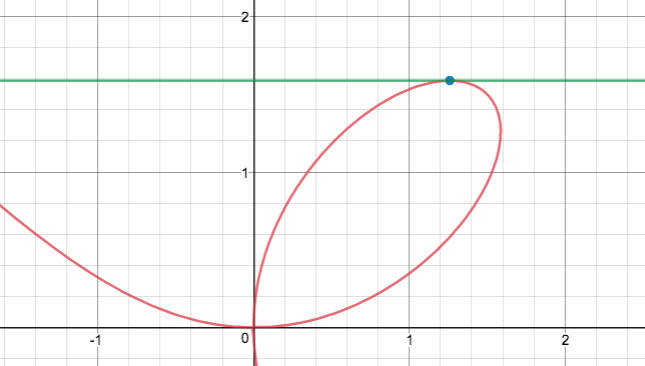
\includegraphics[scale=0.5]{graph7}
\end{center}
As we can see, there is a horizontal line at this point.
Now let's find the vertical tangent line, or when $\frac{dx}{dt}$ is 0.
$$\frac{dx}{dt}=\frac{3-6t^3}{(t^3+1)^2}$$
$$0=\frac{3-6t^3}{(t^3+1)^2}$$
Multiply both sides by the denominator.
$$0=3-6t^3$$
$$6t^3=3$$
$$t=0.793700525984$$
Let's substitute this into the x parametric to find the line at this point.
$$x(0.793700525984)=1.58740105197$$
\begin{center}
    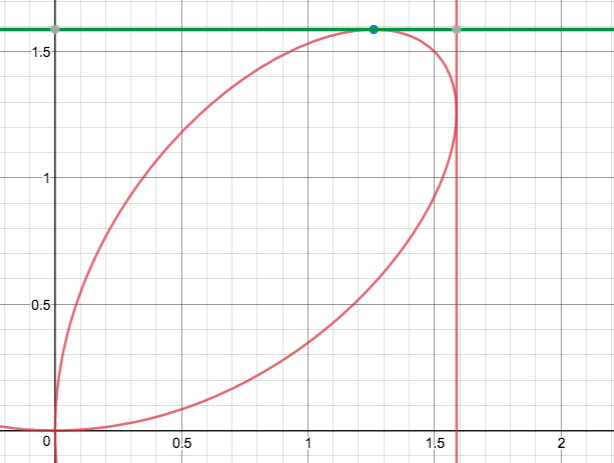
\includegraphics[scale=0.5]{graph8}
\end{center}
As we can see, there is a vertical tangent line at this point, and it is symmetrical to the horizontal tangent line across the $y=x$ line.\\
Now, let's use the point (1.5,1.5) to find the slope of the tangent line at this point. 
$$\frac{1.5^2-1.5}{1.5-1.5^2}=-1$$
\begin{center}
    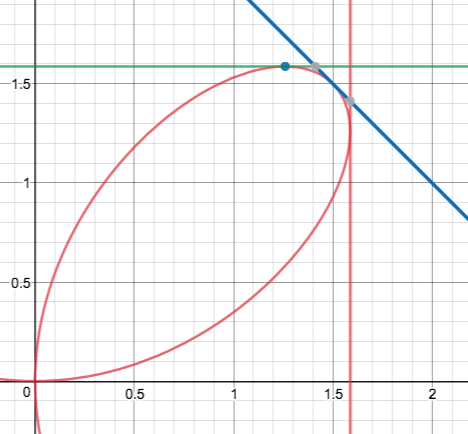
\includegraphics[scale=0.5]{graph9}
\end{center}
As we can see from this image, the tangent line has a slope of -1 and is symmetrically split along the $y=x$ line.
\section*{Finding the Oblique Asymptote}
Since we discovered that the ends of the graph stretch out to approach t=-1, we should explore the slope that these ends appear to approach. They appear to approach a diagonal line, which is also called an oblique asymptote. The best way to understand what the ends of the graph approach is by finding the equation of this asymptote.\\\\
To find the slope of the line that the graph appears to approach, we should find the limit of y' as t approaches -1. We should use y' instead of $\frac{dy}{dx}$ because y' is only in terms of t and will allow us to easily substitute -1 in for t.
$$y'=\frac{2t-t^4}{1-2t^3}$$
$$\lim_{t\to-1}\frac{2t-t^4}{1-2t^3}$$
Let's try directly substituting 1 in for t because it appears to generate a value. Therefore, we won't have to use L'Hopital's Rule.
$$\frac{2-1}{1-2}=-\frac{1}{1}=-1$$
Now we know that -1 is the slope of the tangent line. Since we want to generate the equation of a tangent line in terms of x and y, we substitute our slope in for $\frac{dy}{dx}$ to generate an equation in terms of x and y that we can solve to find the equation of the asymptote.
$$\frac{x^2-y}{x-y^2}=-1$$
Multiply both sides by $x-y^2$
$$x^2-y=-x+y^2$$
Add $x$ to both sides
$$-y+x^2+x=y^2$$
Subtract $y^2$ from both sides
$$-y^2-y+x^2+x=0$$
Divide both sides by -1 to make $y^2$ and $y$ positive value so we can set up a quadratic equation in terms of y. Making $y^2$ positive would make it easier to solve.
$$y^2+y-x^2-x=0$$
Now we should factor a negative 1 out of the x values and group them together. 
$$y^2+y-(x^2+x)=0$$
Since we don't know what $x^2+x$ equals, we can't factor the quadratic and we must put it through the quadratic formula with these values:\\
$a=1$\\
$b=1$\\
$c=x^2+x$\\
Lets use these values to solve using the formula.
$$y=\frac{-1\pm \sqrt{1-4(-x^2-x)}}{2}$$
Multiply both sides by 2.
$$2y=-1\pm \sqrt{4x^2+4x+1}$$
Factor $4x^2+4x+1$
$$2y=-1\pm \sqrt{(2x+1)^2}$$
Now, the square root and the squared sign will cancel each other out.
$$2y=-1\pm 2x+1$$
Since there's a plus or minus sign, we'll have to solve two different equations. First, lets solve the equation for when the sign is a plus.
$$2y=-1+2x+1$$
$$2y=2x$$
Divide both sides by 2.
$$y=x$$
Let's try solving the equation when the sign is a minus.
$$2y=-1-2x-1$$
$$2y=-2x-2$$
Divide both sides by 2.
$$y=-x-1$$
We know that $y=-x-1$ must be the equation of the asymptote because it has a negative slope while $y=x$ doesn't, and the graph shows a negative slope for the asymptote.
\ssection{Area}
\section*{Using Integration to Find the Area Inside the Loop}
To begin to find the area, we'll first have to convert the equation into polar form from rectangular form. To do this, lets substitute $rcos\theta$ in for x and $rsin\theta$ in for y.
$$x^3+y^3=3xy$$
$$(rcos\theta)^3+(rsin\theta)^3=3rcos\theta \cdot rsin\theta$$
Factor out $r^2$ from both sides.
$$r^2(rcos^3\theta +rsin^3\theta)=3r^2cos\theta sin\theta$$
Divide both sides by $r^2$.
$$rcos^3\theta +rsin^3\theta=3cos\theta sin\theta$$
Isolate r.
$$r=\frac{3cos\theta sin\theta}{cos^3\theta +sin^3\theta}$$
The formula for finding polar area is:
$$\frac{1}{2}\int\limits_{\theta_1}^{\theta_2} r^2d\theta$$
So, we have almost all of our information to substitute into the formula. However, we also need to find the $t_1$ and $t_2$ values. The approach to take is to find the area from the origin to the point (1.5,1.5), which is the coordinate of the loop. We'll use the relationship between x,y, and t(shown below) to find the theta values at the origin and at the point (1.5,1.5).
$$tan\theta=(\frac{y}{x})$$
Let's rewrite it so we can easily solve for $\theta$.
$$\theta=arctan(\frac{y}{x})$$
Now, let's substitute in the point (0,0) to find our lower bound.
$$\theta=arctan(\frac{0}{0})=0$$
Now, let's substitute in the point (1.5,1.5) to find our upper bound.
$$\theta=arctan(\frac{1.5}{1.5})$$
$$\theta=arctan(1)$$
Now, we have to think about where on the unit circle the cosine and sine values are the same. This happens at $\frac{\pi}{4}$ so that's our upper bound. We should multiply the numerator and denominator of r by something so that we can integrate r rather easily once it's squared. We're going to multiply it by $\frac{1}{cos^3\theta}$ to simplify it.
$$r=\frac{3cos\theta sin\theta \frac{1}{cos^3\theta}}{(cos^3\theta +sin^3\theta)\frac{1}{cos^3\theta}}$$
Simplify.
$$r=\frac{3\frac{sin\theta}{cos^2\theta}}{1+tan^3\theta}$$
Simplify again.
$$r=\frac{3tan\theta sec\theta}{1+tan^3\theta}$$
This is what we will substitute in for r.
$$2\cdot \frac{1}{2}\int\limits_{0}^{\frac{\pi}{4}}(\frac{3tan\theta sec\theta}{1+tan^3\theta})^2d\theta$$
We have to multiply the formula by 2 because in the integral we're finding one of the two halves of the area and so we need to find the area of the second half as well. Now we'll square r.
$$\int\limits_{0}^{\frac{\pi}{4}}\frac{9tan^2\theta sec^2\theta}{(1+tan^3\theta)^2}d\theta$$
To be able to integrate, we'll have to do u-substitution. Since $tan^3\theta$ is in the denominator, we'll set that equal to u so that we can end up with du in the numerator.
$$u=tan^3\theta$$
$$du=3tan^2\theta sec^2\theta d\theta$$
Now we should move a 3 from the numerator to the outside of the integral so that we can make a clean substitution.
$$3\int\limits_{0}^{\frac{\pi}{4}}\frac{1}{(1+u)^2}du$$
Now we have to be careful. We also have to remember to change the bounds when we do a u-substitution. Since u equals $tan^3\theta$, we'll have to substitute 0 and $\frac{\pi}{4}$ in for theta to get values for the bounds in relation to u.
$$tan^3(\frac{\pi}{4})=1$$
The value of tan at this point is $\frac{\frac{\sqrt{2}}{2}}{\frac{\sqrt{2}}{2}}^3$ which is just 1.
$$tan^3(0)=0$$
The value of tan at this point is $\frac{0}{1}^3$ which is just 0.
$$3\int\limits_{0}^{1}\frac{1}{(1+u)^2}du$$
To be able to integrate, we'll have to do one more u-substitution, this time with z as a variable.
$$u+1=z$$
$$du=dz$$
$$3\int\limits_{0}^{1}\frac{1}{z^2}dz$$
Now we can integrate.
$$3(-\frac{1}{z})\mid_{0}^{1}$$
$$-\frac{3}{z}\mid_{0}^{1}$$
Now we have to subsitute $u+1$ in for $z$.
$$-\frac{3}{u+1}\mid_{0}^{1}$$
Lastly, we have to evaluate the integral from 0 to 1.
$$-\frac{3}{2}--3$$
$$-\frac{3}{2}+\frac{6}{2}=\frac{3}{2}$$
The area inside the loop is 1.5.
\ssection{Conclusion}
\section*{Predicting the Behavior of a Generalized Folium}
Based on what we've seen so far, we can make several conclusions for a general folium.\\\\
1. The area of the loop is $\frac{1}{2}$ of the value in front of $xy$ in the rectangular equation.\\\\
2. Both the x and y coordinates of the loop are $\frac{1}{2}$ of the value in front of $xy$ in the rectangular equation and are equal to the area of the loop.\\\\
3. The slope of the tangent line of the point at the loop is equal to the slope of the oblique asymptote.
\end{document}
